
\documentclass{article}
\usepackage{graphicx}
\usepackage[utf8]{inputenc}
\usepackage{amsmath, amssymb, latexsym}
\usepackage{neuralnetwork}
\usepackage{multicol}
\usepackage{expl3}

\usepackage{pgfplots}
\usepackage{algorithm}
\usepackage[noend]{algpseudocode}
\usepackage{tikz}
\usepackage{nicefrac}
\pgfplotsset{every axis legend/.append style={
at={(0,0)},
anchor=north east}}
\usetikzlibrary{shapes,positioning,intersections,quotes}
\usetikzlibrary{arrows.meta,
                bending,
                intersections,
                quotes,
                shapes.geometric}
                
\definecolor{darkgreen}{rgb}{0.0, 0.6, 0.0}
\definecolor{darkred}{rgb}{0.7, 0.0, 0.0}
\makeatletter
\def\BState{\State\hskip-\ALG@thistlm}
\makeatother
\title{Week 13}
\begin{document}
\pagenumbering{gobble}
\maketitle
\newpage
\pagenumbering{arabic}

\section*{Unsupervised learning}

\begin{itemize}
  \item Try to figure out the structure of the data.
  \item The clustering algorithm organizes data based on data characteristics.
  \item Market segmentation is categorizing clients into different market categories.
  \item Social network analysis.
  \item Computer clusters and data centers are organized for network structure and location.
  \item Understanding galaxy creation through astronomical data analysis.
\end{itemize}

\section*{K-means algorithm}

\begin{itemize}
  \item Would you like an algorithm to automatically arrange data into coherent clusters?
  \item By far the most used clustering algorithm is K-means.
\end{itemize}

~\\
Algorithm overview:

\begin{enumerate}
    \item Assign k locations at random as cluster centroids.
    \item Go through each example and assign each point to one of the k clusters based on which center it is closest to.

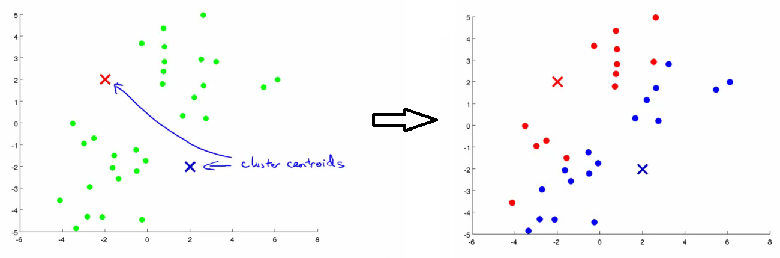
\includegraphics[width=\textwidth]{resources/kclusters_1}

    \item Move to the average of the similarly allocated data-points for each centroid.

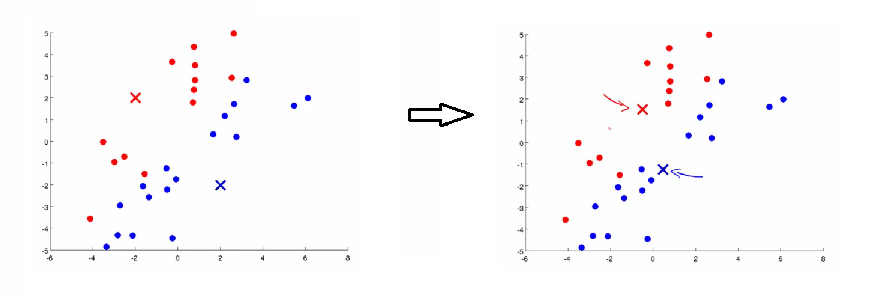
\includegraphics[width=\textwidth]{resources/kclusters_2}

    \item Repeat 2) and 3) until convergence.
\end{enumerate}

\section*{K-means for non-separated clusters}


\begin{itemize}
  \item So far, we've looked at K-means, which has well-defined clusters.
  \item However, K-means is frequently used on datasets with poorly defined clusters.
  \item As an example, consider t-shirt sizes. How large do you make them if you want three sizes (S,M,L)?
  \item As a result, three clusters are formed, even if they are not actually there.
  \item This is an example of market segmentation; create items that are tailored to the demands of your subpopulations.
\end{itemize}

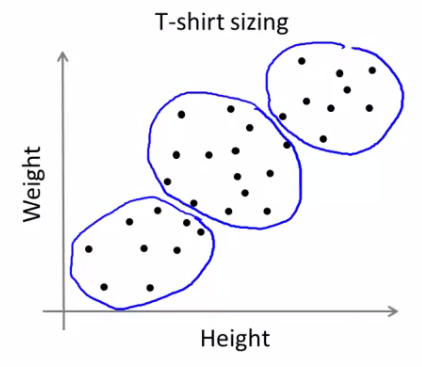
\includegraphics[width=0.5\textwidth]{resources/t_shirt}

\section*{K means optimization objective}

\begin{itemize}
  \item K-means, like the supervised learning functions we've examined, has an optimization goal.
  \item While K-means is running, we keep track of two sets of variables.
  \item $c^i$ is the index of clusters ${1,2, ..., K}$ to which $x^i$ is currently assigned.
  \item $\mu_k$, is the cluster associated with centroid $k$.
  \item  $\mu_c^i$, is the cluster centroid of the cluster to which example $x^i$ has been assigned to.
  \item We may write the optimization objective using this notation:
\end{itemize}

$$J(c^{(1)}, ..., c^{(m)}, \mu_1, ...,\mu_K)=\frac{1}{m}\sum_{i=1}^{m}||x^{(i)}-\mu_{c^{(i)}}||^2$$

~\\
i.e. squared distances between training example $x^i$ and the cluster centroid to which $x^i$ has been assigned to.

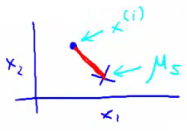
\includegraphics[width=0.5\textwidth]{resources/cost_cluster}

~\\
When we look at the k-means method:

\begin{itemize}
  \item The cluster assigned step is minimizing $J(...)$ with respect to $c_1, c_2 ... c_i$ i.e. find the centroid closest to each example. Doesn't change the centroids themselves.
  \item The move centroid step. We can show this step is choosing the values of $\mu$ which minimizes $J(...)$ with respect to $\mu$.
  \item So, we're partitioning the algorithm into two parts: First part minimizes the $c$ variables. Second part minimizes the $J$ variables.
\end{itemize}

\section*{Random initialization}
Depending on the starting setting, K means might converge to different solutions.

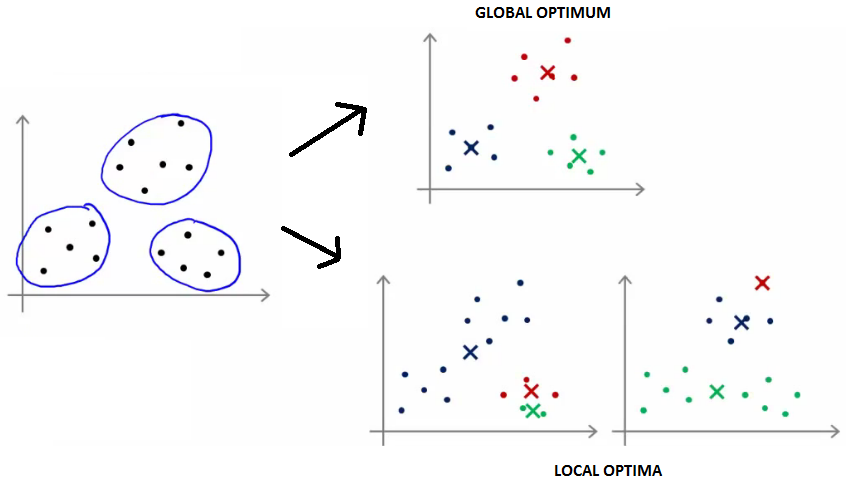
\includegraphics[width=\textwidth]{resources/optimum_cluster}

\begin{itemize}
  \item Randomly initialize K-means.
  \item For each n (e.g. 100) random initialization run K-means.
  \item Then compute the distortion on the set of cluster assignments and centroids at convergent.
  \item End with n ways of cluster the data.
  \item Pick the clustering which gave the lowest distortion.
\end{itemize}

\section*{Elbow method}

\begin{itemize}
  \item How do we choose the number of clusters K?
  \item Vary K and compute cost function at a range of K values.
  \item $J(...)$'s minimum value should decrease as K rises (i.e. you decrease the granularity so centroids can better optimize).
  \item Look for the "elbow" on the graph ($K$ vs $J()$).
\end{itemize}

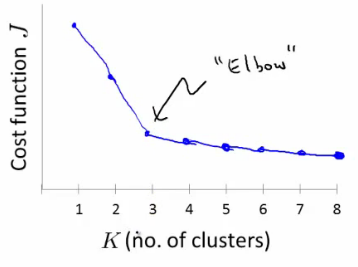
\includegraphics[width=0.47\textwidth]{resources/elbow}

\end{document}
